\documentclass[a4paper,12pt]{article}
\usepackage{tikz}
\usetikzlibrary{arrows,positioning}
\begin{document}

We are given the expression \texttt{(list 1 (list 2 (list 3 4)))}

\bigskip The result printed by the interpreter (In SICP mode) \\
\texttt{(mcons 1 (mcons (mcons 2 (mcons (mcons 3 (mcons 4 '())) '())) '()))}

\bigskip In racket mode
\texttt{'(1 (2 (3 4)))}

\bigskip The box and pointer structure \\

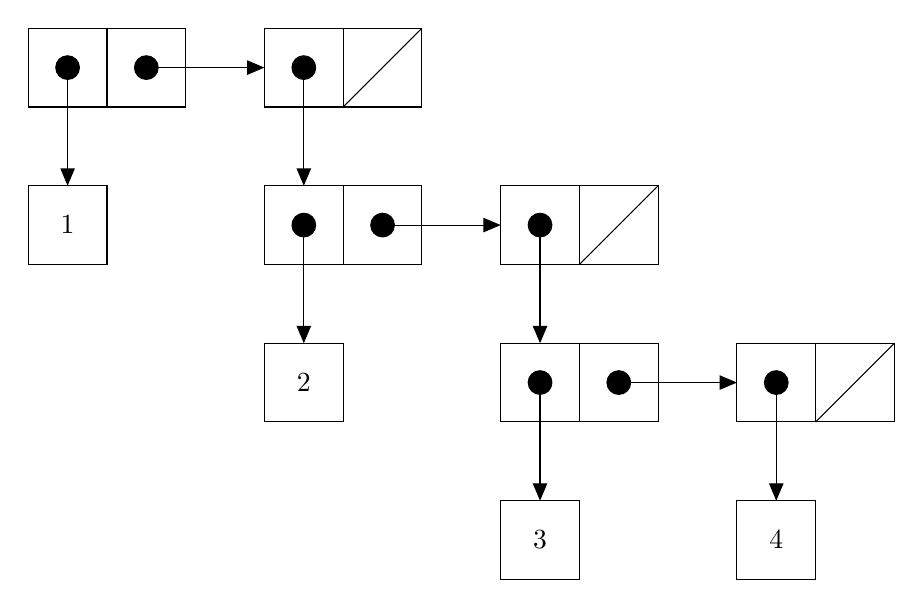
\begin{tikzpicture}
\draw (0, 0) rectangle (1, 1);
\draw (1, 0) rectangle (2, 1);
\draw (3, 0) rectangle (4, 1);
\draw (4, 0) rectangle (5, 1);
\draw [fill=black] (0.5, 0.5) circle [radius=0.15];
\draw [fill=black] (1.5, 0.5) circle [radius=0.15];
\draw [fill=black] (3.5, 0.5) circle [radius=0.15];
\draw [arrows={-triangle 45}] (1.5, 0.5) -- (3, 0.5);
\draw [arrows={-triangle 45}] (0.5, 0.5) -- (0.5, -1);
\draw [arrows={-triangle 45}] (3.5, 0.5) -- (3.5, -1);
\draw (4, 0) -- (5, 1);
\node at (0.5, -1.5) {1};

\draw (0, -2) rectangle (1, -1);
\draw (3, -2) rectangle (4, -1);
\draw (4, -2) rectangle (5, -1);
\draw (6, -2) rectangle (7, -1);
\draw (7, -2) rectangle (8, -1);
\draw [fill=black] (3.5, -1.5) circle [radius=0.15];
\draw [fill=black] (4.5, -1.5) circle [radius=0.15];
\draw [fill=black] (6.5, -1.5) circle [radius=0.15];
\draw [arrows={-triangle 45}] (4.5, -1.5) -- (6, -1.5);
\draw [arrows={-triangle 45}] (3.5, -1.5) -- (3.5, -3);
\draw [arrows={-triangle 45}] (6.5, -1.5) -- (6.5, -3);
\draw (7, -2) -- (8, -1);
\node at (3.5, -3.5) {2};

\draw (3, -4) rectangle (4, -3);
\draw (6, -4) rectangle (7, -3);
\draw (7, -4) rectangle (8, -3);
\draw (9, -4) rectangle (10, -3);
\draw (10, -4) rectangle (11, -3);
\draw [fill=black] (6.5, -3.5) circle [radius=0.15];
\draw [fill=black] (7.5, -3.5) circle [radius=0.15];
\draw [fill=black] (9.5, -3.5) circle [radius=0.15];
\draw [arrows={-triangle 45}] (7.5, -3.5) -- (9, -3.5);
\draw [arrows={-triangle 45}] (6.5, -3.5) -- (6.5, -5);
\draw [arrows={-triangle 45}] (9.5, -3.5) -- (9.5, -5);
\draw (10, -4) -- (11, -3);

\draw (6, -6) rectangle (7, -5);
\draw (9, -6) rectangle (10, -5);
\node at (6.5, -5.5) {3};
\node at (9.5, -5.5) {4};

\end{tikzpicture}

\bigskip The tree structure
\begin{center}
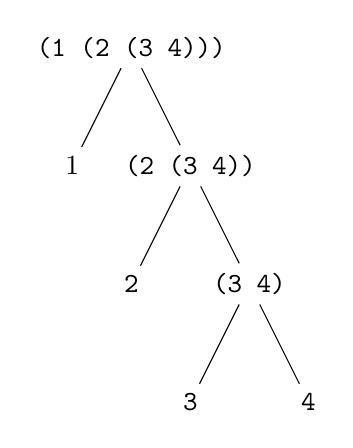
\begin{tikzpicture}
[level 2/.style={sibling distance=15mm}]
\node {\texttt{(1 (2 (3 4)))}}
	child {node {1}}
	child {node {\texttt{(2 (3 4))}}
		child {node {\texttt{2}}}
		child {node {\texttt{(3 4)}}
			child {node {\texttt{3}}}
			child {node {\texttt{4}}}}};
\end{tikzpicture}
\end{center}

\end{document}